\documentclass{book}
\usepackage{commeunjeustyle}

\begin{document}

\chapter*{Groupes}



\begin{Texte}%label=introduction
Le concept de groupe fit son apparition dans l'étude des équations polynomiales. En effet, c'est Évariste Galois qui, durant les années 1830, utilisa pour la première fois le terme « groupe » dans un sens technique similaire à ce qui est utilisé de nos jours, faisant de lui un des fondateurs de la théorie des groupes. \\
Depuis le lycée, la résolution des équations de degré $2$ du type
$ax^2+bx+c=0$ n'a plus de mystère. On peut aussi déterminer des solutions pour les équation de degré $3$, $ax^3+bx^2+cx+d=0$, et de degré $5$, $ax^4+bx^3+cx^2+dx+e=0$, cependant le 
Cependant existent-ils des solutions pour les équations de degré  $5$. La réponse fut apportée par Galois : il n'existe pas en général une telle
 formule. La notion de groupe est introduit dans la démonstration. \\
Suite à des contributions d'autres domaines des mathématiques, comme la théorie des nombres et la géométrie, la notion de groupe fut généralisée et plus fermement établie autour des années 1870.\\
\end{Texte}
\section{Groupe}
\subsection{Définition}
\begin{Definition}[Groupe]
Un \defi{groupe} est un couple $(G,\ast)$ où $G$ est un ensemble et $\ast$ une loi de composition interne sur $G$ associative, admettant un neutre et pour laquelle tout élément de $G$ admet un symétrique pour la loi $\ast$.\\
Un groupe est dit \defi{abélien} ou \defi{commutatif} si la loi $\ast$ est de plus commutative.
\end{Definition}
\begin{Remarque}
Lors de l'introduction d'un groupe $(G,*)$, on omet de mentionner la loi $*$ afin d'alléger les notations.\\
L'ensemble $G$ ne peut pas être vide car il contient au moins l'élément neutre noté $e$.\\
L'inverse d'un élément $x$ est noté $x^{-1}$.
\end{Remarque}
\begin{Proposition}[Groupes de référence]
$(\Z, +), (\Q, +), (\R, +)$ et  $(\C, +)$  sont des groupes commutatifs.\\
$(\Q^*, \times), (\R^*, \times)$ et  $(\C^*,\times)$  sont des groupes commutatifs.\\ 
\end{Proposition}
\begin{Demonstration}
Les hypothèses à vérifier ont été énoncées dans la section précédente.
\end{Demonstration}
\begin{Exemple}[Groupe diédral]
Une symétrie transforme une figure du plan en elle-même. Pour le carré, l'ensemble des symétries forme un groupe constitué de 8 éléments :
\begin{itemize}
\item l'application identité, laissant tout inchangé, 
\item les rotations de 90° , 180° et 270° vers la droite de Le centre le point d'intersection des diagonales du carré,
\item les réflexions ayant pour axes les médiatrices des côtés du carré  ou ses diagonales .
\end{itemize}

\begin{center}
\begin{Figure}
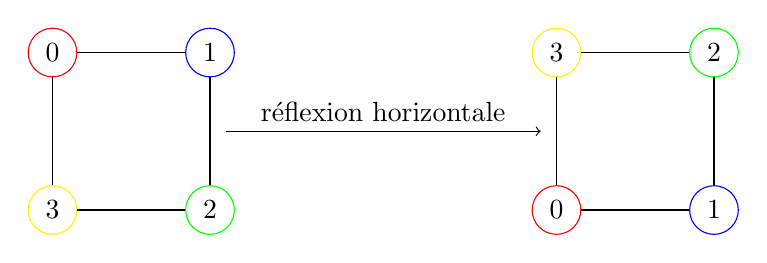
\begin{tikzpicture}
\node[draw=red,circle](A) at  (0,0) {$0$};
\node[draw=blue,circle](B) at (2,0) {$1$};
\node[draw=green,circle](C) at (2,-2) {$2$};
\node[draw=yellow,circle](D) at (0,-2) {$3$};
\draw (A) -- (B);
\draw (B) -- (C);
\draw (C) -- (D);
\draw (D) -- (A);
\draw [->] (2.2,-1) -- (6.2,-1) node [midway, above] {réflexion horizontale};
\node[draw=red,circle](A) at  (6.4,-2) {$0$};
\node[draw=blue,circle](B) at (8.4,-2) {$1$};
\node[draw=green,circle](C) at (8.4,0) {$2$};
\node[draw=yellow,circle](D) at (6.4,0) {$3$};
\draw (A) -- (B);
\draw (B) -- (C);
\draw (C) -- (D);
\draw (D) -- (A);
\end{tikzpicture}\\
\begin{Titre}
 Les sommets du carré sont identifiés par une couleur et une nombre.
\end{Titre}
\end{Figure}
\end{center}
Deux symétries quelconques peuvent être composées, c'est-à-dire appliquées l'une après l'autre.
\end{Exemple}

\begin{Exemple}[Permutation, groupe symétrique] Soit $E$ un ensemble non vide. On appelle \defi{permutation} de E toute
bijection de $E$ sur $E$, et groupe symétrique de $E$ l'ensemble des permutations de $E$.
\end{Exemple}


\subsection{Sous-groupes}
\begin{Definition}[Sous-Groupe]
Soit $(G, *)$ un groupe et $H$ une partie de $G$.\\
$(H, *)$ est un \defi{sous-groupe} de $(G, *)$  si $H$ est stable pour $*$ et, muni de la loi induite, est un groupe.
\end{Definition}
\begin{Proposition}[Caractérisation des sous-groupes]
Soit $(G, *)$ un groupe et $H$ une partie de $G$.\\
H est un sous-groupe de G si et seulement si:
\begin{itemize}
  \item $e_G \in H$,
  \item pour tout $x, y \in H$, on a $x * y \in H$,
  \item pour tout $x \in H$, on a $x^{-1} \in H$.
\end{itemize}
\end{Proposition}
\begin{Exemple}
\begin{itemize}
  \item $(\R^*_+,\times)$ est un sous-groupe de $(\R^*,\times)$.
En effet :
  \begin{itemize}
     \item $1 \in \R^*_+$,
     \item si $x,y \in \R^*_+$ alors $x\times y \in \R^*_+$,
     \item si $x \in \R^*_+$ alors $x^{-1} = \frac 1 x \in \R^*_+$.
   \end{itemize}
  \item $(\mathbb{U},\times)$ est un sous-groupe de $(\C^*,\times)$, où
$\mathbb{U} = \{ z \in \C : |z|=1 \}$. 
En effet :
  \begin{itemize}
     \item $|\overbrace{1}^{\in\C}|=\overbrace{1}^{\in\R}$ donc $1\in\mathbb{U}$,
     \item Si $z,z' \in \mathbb{U}$ alors $|zz'|=|z||z'|=1$ d'où  $zz' \in \mathbb{U}$,
     \item si $z \in \mathbb{U}$ alors $|z^{-1}|=\left|\frac{1}{z}\right|=\frac{1}{|z|}=1$ d'où  $z^{-1} \in \mathbb{U}$,
   \end{itemize}
  \item $(\Z,+)$ est un sous-groupe de $(\R,+)$.
  \item $\{e\}$ et $G$ sont les \defi{sous-groupes triviaux} du groupe $G$.
  \item L'ensemble $\mathcal{R}$ des rotations du plan dont le centre est à l'origine
est un sous-groupe du groupe des isométries $\mathcal{I}$.
\end{itemize}
\end{Exemple}
%TODO DEMO

%---------------------------------------------------------------
\subsection{Sous-groupes de $\Z$}
\begin{Definition}[$n\Z$]
L'ensemble $n\Z$ désigne l'ensemble des multiples de $n$ :
$$n\Z = \{ k\cdot n : k \in \Z\}.$$
Par exemple:
\begin{itemize}
  \item $2\Z = \{\ldots, -4,-2,0,+2,+4,+6,\ldots\}$ est l'ensemble des entiers pairs,
  \item $7\Z =  \{\ldots, -14,-7,0,+7,+14,+21,\ldots\}$ est l'ensemble des multiples de $7$.
\end{itemize}
\end{Definition}
\begin{Proposition}
Les sous-groupes de $(\Z,+)$ sont les $n\Z$, pour $n\in \Z$.
\end{Proposition}

\begin{Demonstration}
\begin{itemize}
\item Soit $n \in \Z$. L'ensemble $n\Z$ est ainsi un sous-groupe de $(\Z,+$ en effet : 
\begin{itemize}
 \item $n\Z \subset \Z$,
 \item l'élément neutre $0$ appartient à $n\Z$,
 \item pour $x = kn$ et $y=k'n$ des éléments de $n\Z$ alors $x+y = (k+k')n$ est aussi un
élément de $n\Z$,
 \item enfin si $x=kn$ est un élément de $n\Z$ alors $-x=(-k)n$ est aussi un élément de $n\Z$.
\end{itemize}
\item Réciproquement soit $H$ un sous-groupe de $(\Z,+)$.
Si $H=\{0\}$ alors $H = 0\Z$ et c'est fini. Sinon $H$ contient au moins un élément non-nul et positif (puisque tout élément est accompagné de son opposé) et
notons
$$n=\min \{ h > 0 : h \in H \}.$$
\begin{itemize}
 \item $n\Z \subset H : $ Comme $n\in H$ alors $-n \in H$, $2n=n+n \in H$, et plus généralement pour $k \in \Z$ alors $kn \in H$.
 \item $ H\subset n\Z : $
Soit $h \in H$. Écrivons la division euclidienne :
$$h = kn + r,\quad \text{avec } k,r \in \Z  \ \text{ et } \  0 \le r < n.$$
Mais $h\in H$ et $kn \in H$ donc
$r= h - kn \in H$. Nous avons un entier $r \ge 0$ qui est un élément de
$H$ et strictement plus petit que $n$. Par la définition de $n$, nécessairement
$r=0$. Autrement dit $h=kn$ et donc $h\in n\Z$.
\end{itemize}
Conclusion $H=n\Z$.
\end{itemize}










\end{Demonstration}
%---------------------------------------------------------------
\section{Groupe des permutations}
\section{Definition}
\begin{DefinitionProposition}
Une bijection de $\{1,2,\ldots,n\}$ (dans lui-même) s'appelle une \defi{permutation}
L'ensemble des permutations  est un groupe, noté $(\mathcal{S}_n,\circ)$.\\
Le groupe $(\mathcal{S}_n,\circ)$ s'appelle le \defi{groupe des permutations}
(ou le \defi{groupe symétrique}).
\end{DefinitionProposition}

\begin{Demonstration}

\begin{enumerate}
  \item La composition de deux bijections de $\{1,2,\ldots,n\}$ est une bijection de $\{1,2,\ldots,n\}$.
  \item La loi est associative (par l'associativité de la composition des fonctions).
  \item L'élément neutre est l'identité.
  \item L'inverse d'une bijection $f$ est sa bijection réciproque $f^{-1}$.
\end{enumerate}
\end{Demonstration}


\begin{Lemme}
Le cardinal de $\mathcal{S}_n$ est $n!$~.
\end{Lemme}

\begin{Demonstration}
La preuve est simple. Pour l'élément $1$, son image appartient à $\{1,2,\ldots,n\}$ donc nous avons $n$ choix.
Pour l'image de $2$, il ne reste plus que $n-1$ choix ($1$ et $2$ ne doivent pas avoir la même image car
notre application est une bijection).
Ainsi de suite... Pour l'image du dernier élément $n$ il ne reste qu'une possibilité.
Au final
il y a $n\times(n-1)\times \cdots \times 2 \times 1 = n!$ façon de construire des bijections
de  $\{1,2,\ldots,n\}$.
\end{Demonstration}
%---------------------------------------------------------------
\subsection{Notation et exemples}
\begin{Vocabulaire}
Décrire une permutation $f : \{1,2,\ldots,n\} \longrightarrow \{1,2,\ldots,n\}$ équivaut à donner
les images de chaque $i$ allant de $1$ à $n$.
Nous notons donc $f$ par
$$\left[\begin{matrix}
 1    & 2    & \cdots & n \\
 f(1) & f(2) & \cdots & f(n) \\
        \end{matrix}
 \right]
$$

Par exemple la permutation de $\mathcal{S}_7$ notée
  $$
    \begin{tikzpicture}[thick]
      \matrix(M)[inner sep=0pt, nodes={inner sep=3pt},matrix of math nodes, left delimiter=[,right delimiter={]}, font=\small]{
        1 & 2 & 3 & 4 & 5 & 6 & 7 \\
        3 & 7 & 5 & 4 & 6 & 1 & 2 \\
      };
      \draw ([shift={(.8em,.8em)}]M.east) edge[colordef,bend left=45,{[scale=.7]|}->] node[right=-2pt,font=\small]{$f$}([shift={(.8em,-.8em)}]M.east);
    \end{tikzpicture}
  $$
est la bijection $f : \{1,2,\ldots,7\} \longrightarrow \{1,2,\ldots,7\}$
définie par $f(1)= 3$, $f(2)=7$, $f(3)=5$, $f(4)=4$, $f(5)=6$, $f(6)=1$, $f(7)=2$.
C'est bien une bijection car chaque nombre de $1$ à $7$ apparaît une fois et une seule
sur la deuxième ligne.\\

L'élément neutre du groupe est l'identité $I_d$ ; pour $\mathcal{S}_7$ c'est donc
$\left[\begin{smallmatrix}
 1 & 2 & 3 & 4 & 5 & 6 & 7 \\
 1 & 2 & 3 & 4 & 5 & 6 & 7 \\
        \end{smallmatrix} \right]
$.

Il est facile de calculer la composition de deux permutations $f$ et $g$ avec cette notation.
Si
$f =\left[\begin{smallmatrix}
 1 & 2 & 3 & 4 & 5 & 6 & 7 \\
 3 & 7 & 5 & 4 & 6 & 1 & 2 \\
        \end{smallmatrix} \right]
$
et
$g = \left[\begin{smallmatrix}
 1 & 2 & 3 & 4 & 5 & 6 & 7 \\
 4 & 3 & 2 & 1 & 7 & 5 & 6 \\
        \end{smallmatrix} \right]
$
alors $g\circ f$ s'obtient en superposant la permutation $f$ puis $g$
$$g\circ f
= \begin{tikzpicture}[thick,baseline={([yshift=-.3em]M.center)}]
    \matrix(M)[inner sep=0pt, nodes={inner sep=3pt},matrix of math nodes, left delimiter=[,right delimiter={]}, font=\small]{
      1 & 2 & 3 & 4 & 5 & 6 & 7 \\
      3 & 7 & 5 & 4 & 6 & 1 & 2 \\
      2 & 6 & 7 & 1 & 5 & 4 & 3 \\
    };
    \draw[colordef] (M.east) -- (M.west);
    \draw ([shift={(1em,1.6em)}]M.east) edge[colordef,{[scale=.7]|}->] node[right=-2pt,font=\small]{$f$}([shift={(1em,0em)}]M.east);
    \draw ([shift={(1em,0em)}]M.east) edge[colordef,{[scale=.7]|}->] node[right=-2pt,font=\small]{$g$}([shift={(1em,-1.6em)}]M.east);
    \draw ([shift={(1.7em,1.6em)}]M.east) edge[colordef,bend left=45,{[scale=.7]|}->] node[right=-2pt,font=\small]{$f\circ g$}([shift={(1.7em,-1.6em)}]M.east);
  \end{tikzpicture}
 = \left[\begin{matrix}
 1 & 2 & 3 & 4 & 5 & 6 & 7 \\
 2 & 6 & 7 & 1 & 5 & 4 & 3
        \end{matrix} \right]
$$
ensuite on élimine la ligne intermédiaire du milieu et donc $g\circ f$ se note
$\left[\begin{smallmatrix}
 1 & 2 & 3 & 4 & 5 & 6 & 7 \\
 2 & 6 & 7 & 1 & 5 & 4 & 3
        \end{smallmatrix} \right]
$.

Il est tout aussi facile de calculer l'inverse d'une permutation :
il suffit d'échanger les lignes du haut et du bas et de réordonner le tableau.
Par exemple l'inverse de
$$
  f=
    \begin{tikzpicture}[thick,baseline=(M.center)]
      \matrix(M)[inner sep=0pt, nodes={inner sep=3pt},matrix of math nodes, left delimiter=[,right delimiter={]}, font=\small]{
        1 & 2 & 3 & 4 & 5 & 6 & 7 \\
        3 & 7 & 5 & 4 & 6 & 1 & 2 \\
      };
      \draw ([shift={(.8em,.8em)}]M.east) edge[colordef,bend left=45,<-{[scale=.7]|}] node[right=-2pt,font=\small]{$f^{-1}$}([shift={(.8em,-.8em)}]M.east);
    \end{tikzpicture}
$$
se note
 $f^{-1} = \left[ \begin{smallmatrix}
 3 & 7 & 5 & 4 & 6 & 1 & 2 \\
 1 & 2 & 3 & 4 & 5 & 6 & 7 \\
        \end{smallmatrix} \right]
$
ou plutôt après réordonnement
 $\left[\begin{smallmatrix}
 1 & 2 & 3 & 4 & 5 & 6 & 7 \\
 6 & 7 & 1 & 4 & 3 & 5 & 2 \\
        \end{smallmatrix} \right]
$.
\end{Vocabulaire}

%---------------------------------------------------------------
\subsection{Le groupe $\mathcal{S}_3$}

Nous allons étudier en détails le groupe $\mathcal{S}_3$ des permutations de $\{1,2,3\}$.
Nous savons que $\mathcal{S}_3$ possède $3!=6$ éléments que nous énumérons :
\begin{itemize}
 \item $I_d = \left[\begin{smallmatrix}
 1 & 2 & 3 \\
 1 & 2 & 3 \\
        \end{smallmatrix} \right]
$ l'identité,

 \item $\tau_1 = \left[\begin{smallmatrix}
 1 & 2 & 3 \\
 1 & 3 & 2 \\
        \end{smallmatrix} \right]
$ une transposition,

 \item $\tau_2 = \left[\begin{smallmatrix}
 1 & 2 & 3 \\
 3 & 2 & 1 \\
        \end{smallmatrix} \right]
$ une deuxième transposition,

 \item $\tau_3 = \left[\begin{smallmatrix}
 1 & 2 & 3 \\
 2 & 1 & 3 \\
        \end{smallmatrix} \right]
$ une troisième transposition,

 \item $\sigma = \left[\begin{smallmatrix}
 1 & 2 & 3 \\
 2 & 3 & 1 \\
        \end{smallmatrix} \right]
$ un cycle,


 \item $\sigma^{-1} = \left[\begin{smallmatrix}
 1 & 2 & 3 \\
 3 & 1 & 2 \\
        \end{smallmatrix} \right]
$ l'inverse du cycle précédent.
\end{itemize}

Donc $\mathcal{S}_3 = \{I_d,\tau_1,\tau_2,\tau_3,\sigma,\sigma^{-1}\}$.


\bigskip

Calculons $\tau_1 \circ \sigma$ et $\sigma \circ \tau_1$ :
$$\tau_1 \circ \sigma
=\left[\begin{smallmatrix}
 1 & 2 & 3 \\
 2 & 3 & 1 \\
 3 & 2 & 1 \\
        \end{smallmatrix} \right]
= \left[\begin{smallmatrix}
 1 & 2 & 3 \\
 3 & 2 & 1 \\
        \end{smallmatrix} \right]
= \tau_2
\quad \text{et} \quad
\sigma \circ \tau_1
= \left[\begin{smallmatrix}
 1 & 2 & 3 \\
 1 & 3 & 2 \\
 2 & 1 & 3 \\
        \end{smallmatrix} \right]
= \left[\begin{smallmatrix}
 1 & 2 & 3 \\
 2 & 1 & 3 \\
        \end{smallmatrix} \right]
= \tau_3.
 $$

Ainsi $\tau_1 \circ \sigma = \tau_2$ est différent de $\sigma \circ \tau_1=\tau_3$,
ainsi le groupe $\mathcal{S}_3$ n'est pas commutatif. Et plus généralement :
\begin{Lemme}
Pour $n\ge 3$, le groupe $\mathcal{S}_n$ n'est pas commutatif.
\end{Lemme}



\bigskip

Nous pouvons calculer la table du groupe $\mathcal{S}_3$
\begin{Figure}
\centering
\begin{tabular}{c||c|c|c|c|c|c}
$g$ $\circ$ $f$  & $I_d$ &$\tau_1$
 & $\tau_2$ & $\tau_3$
&  $\sigma$ & $\sigma^{-1}$ \\ \hline\hline
$I_d$ & $I_d$ & $\tau_1$ & $\tau_2$ & $\tau_3$ & $\sigma$ & $\sigma^{-1}$ \\ \hline

$\tau_1$ & $\tau_1$ & $I_d$ & $\sigma$ & $\sigma^{-1}$ & $\tau_1 \circ \sigma = \tau_2$ & $\tau_3$ \\ \hline

$\tau_2$ & $\tau_2$  & $\sigma^{-1}$ & $I_d$ & $\sigma$ & $\tau_3$ & $\tau_1$ \\ \hline

$\tau_3$ & $\tau_3$ & $\sigma$ & $\sigma^{-1}$ & $I_d$ & $\tau_1$ & $\tau_2$ \\ \hline

$\sigma$ & $\sigma$ &$\sigma \circ \tau_1=\tau_3$ & $\tau_1$ & $\tau_2$ & $\sigma^{-1}$ & $I_d$ \\ \hline

$\sigma^{-1}$ & $\sigma^{-1}$ & $\tau_2$ & $\tau_3$ & $\tau_1$ & $I_d$ & $\sigma$ \\
\end{tabular}\\
Table du groupe $\mathcal{S}_3$
\end{Figure}

Comment avons-nous rempli cette table ? Nous avons déjà calculé
\textcolor{red}{$\tau_1 \circ \sigma = \tau_2$} et
\textcolor{orange}{$\sigma \circ \tau_1=\tau_3$}.
Comme $f\circ I_d = f$ et $I_d \circ f = f$ il est facile de remplir la première colonne noire
ainsi que la première ligne noire. Ensuite il faut faire les calculs !

On retrouve ainsi que $\mathcal{S}_3 = \{I_d,\tau_1,\tau_2,\tau_3,\sigma,\sigma^{-1}\}$ est un groupe :
en particulier la composition de deux permutations de la liste reste une permutation de la liste.
On lit aussi sur la table l'inverse de chaque élément, par exemple sur la ligne de $\tau_2$
on cherche à quelle colonne on trouve l'identité, c'est la colonne de $\tau_2$. Donc l'inverse de $\tau_2$
est lui-même.


%---------------------------------------------------------------
\subsection{Groupe des isométries du triangle}

Soit $(ABC)$ un triangle équilatéral.
Considérons l'ensemble des isométries du plan qui préservent le triangle, c'est-à-dire
que l'on cherche toutes les isométries $f$ telles que $f(A) \in \{A,B,C\}$,
$f(B) \in \{A,B,C\}$, $f(C) \in \{A,B,C\}$.
On trouve les isométries suivantes :
l'identité $I_d$, les réflexions $t_1, t_2, t_3$ d'axes $\mathcal{D}_1, \mathcal{D}_2,\mathcal{D}_3$,
la rotation $s$ d'angle $\frac{2\pi}{3}$ et la rotation $s^{-1}$ d'angle $-\frac{2\pi}{3}$
(de centre $O$).


\begin{tikzpicture}[scale=2]

      \coordinate (A) at (90:1);
      \coordinate (B) at (210:1);
      \coordinate (C) at (330:1);
      \coordinate (O) at (0,0);


        \draw[thick, color=colorprop] (A)--(B)--(C)--cycle;

       \fill (A) circle (1pt);
       \fill (B) circle (1pt);
       \fill (C) circle (1pt);

       \node at (A) [left] {$A$};
       \node at (B) [below left] {$B$};
       \node at (C) [below right] {$C$};

       \fill (O) circle (1pt);
       \node at (O) [below] {$O$};

%\beameronly{\pause}

% Les rotations

       {
      \draw (A)--++(-90:01);
      \draw (B)--++(30:1);
      \draw (C)--++(150:1);

   \draw[->] (90:0.25) arc(90:210:0.25);
    \node at (150:0.25) [below left] {$+\frac{2\pi}{3}$};


   \draw[->] (90:0.2) arc(90:-30:0.2);
    \node at (30:0.20) [below right] {$-\frac{2\pi}{3}$};
}



% Les reflexions

       {
     \draw (A)--++(-90:1.8);
     \draw (B)--++(30:2);
      \draw (C)--++(150:2);

     \node at (-90:0.8) [left] {$\mathcal{D}_1$};
      \node at (30:1) [right] {$\mathcal{D}_2$};
      \node at (150:1) [left] {$\mathcal{D}_3$};
}
\end{tikzpicture}

\begin{Proposition}
L'ensemble des  isométries d'un triangle équilatéral, muni de la composition, forme un groupe.
Ce groupe est isomorphe à $(\mathcal{S}_3,\circ)$.
\end{Proposition}

L'isomorphisme est juste l'application qui à $t_i$ associe $\tau_i$,
à $s$ associe $\sigma$ et à $s^{-1}$ associe $\sigma^{-1}$.


%---------------------------------------------------------------
\subsection{Décomposition en cycles}

\begin{itemize}
  \item Nous allons définir ce qu'est un \defi{cycle}\index{cycle} :
c'est une permutation $\sigma$ qui fixe un certain nombre d'éléments ($\sigma(i)=i$)
et dont les éléments non fixés sont obtenus par itération : $j, \sigma(j),\sigma^2(j),\ldots$
C'est plus facile à comprendre sur un exemple :
$$
\sigma = \left[\begin{matrix}
 1 & \mathbf{2} & 3 & \mathbf{4} & \mathbf{5} & 6 & 7 & \mathbf{8} \\
 1 & \mathbf{8} & 3 & \mathbf{5} & \mathbf{2} & 6 & 7 & \mathbf{4} \\
 \end{matrix} \right]
$$
est un cycle : les éléments $1, 3, 6, 7$ sont fixes,
les autres s'obtiennent comme itération de $2$ :
$2 \mapsto \sigma(2)=8 \mapsto \sigma(8)=\sigma^2(2)=4 \mapsto \sigma(4)=\sigma^3(2) =  5$,
ensuite on retrouve $\sigma^4(2)=\sigma(5)=2$.


  \item Nous noterons ce cycle par
    $$
      \begin{tikzpicture}
        \matrix(M)[matrix of math nodes, left delimiter=(,right delimiter=), inner sep=1pt, column sep=1em]
          {2 & 8 & 4 & 5\\};
        \path[thick,colorprop]
          foreach \i [evaluate={\j=int(\i+1)}] in {1,2,3}{
            (M-1-\i.280) edge[bend right,->] (M-1-\j.255)}
          (M-1-4.north west) edge[bend right=20,->] (M-1-1.north east);
      \end{tikzpicture}
    $$

Il faut comprendre cette notation ainsi : l'image de $2$ est $8$,
l'image de $8$ est $4$, l'image de $4$ est $5$, l'image de $5$ est $2$.
Les éléments qui n'apparaissent pas (ici $1, 3, 6, 7$) sont fixes.
On aurait pu aussi noter ce même cycle par : $(8\ 4\ 5\ 2)$, $(4\ 5\ 2\ 8)$ ou $(5\ 2\ 8\ 4)$.

  \item Pour calculer l'inverse on renverse les nombres : l'inverse de $\sigma = (2\ 8\ 4\ 5)$ est
$\sigma^{-1}=(5\ 4\ 8\ 2)$.

  \item Le \defi{support}\index{support} d'un cycle sont les éléments qui ne sont pas fixes : le support de $\sigma$ est $\{2, 4, 5, 8\}$.
La \defi{longueur} (ou l'\defi{ordre}) d'un cycle est le nombre d'éléments qui ne sont pas fixes
(c'est donc le cardinal du support).
Par exemple $(2\ 8\ 4\ 5)$ est un cycle de longueur $4$.

  \item Autres exemples :
$
\sigma = \left[\begin{smallmatrix}
 1 & 2 & 3 \\
 2 & 3 & 1 \\
        \end{smallmatrix} \right]
= (1\ 2\ 3)$ est un cycle de longueur $3$ ;
$
\tau = \left[\begin{smallmatrix}
 1 & 2 & 3 & 4 \\
 1 & 4 & 3 & 2 \\
        \end{smallmatrix} \right]
= (2\ 4)$ est un cycle de longueur $2$, aussi appelé une \defi{transposition}\index{transposition}.

  \item Par contre
$f =\left[\begin{smallmatrix}
 1 & 2 & 3 & 4 & 5 & 6 & 7 \\
 7 & 2 & 5 & 4 & 6 & 3 & 1 \\
        \end{smallmatrix} \right]
$ n'est pas un cycle ; il s'écrit comme la composition de deux cycles
$f = (1\ 7) \circ (3\ 5\ 6)$. Comme les supports de $(1\ 7)$ et $(3\ 5\ 6)$ sont disjoints
alors on a aussi $f = (3\ 5\ 6) \circ (1\ 7)$.

\end{itemize}


\medskip

Ce dernier point fait partie d'un résultat plus général que nous admettons :
\begin{Theoreme}
Toute permutation de $\mathcal{S}_n$ se décompose en composition
de cycles à supports disjoints.
De plus cette décomposition est unique.
\end{Theoreme}

Pour l'unicité il faut comprendre : unique à l'écriture de chaque cycle près
(exemple : $(3\ 5\ 6)$ et $(5\ 6\ 3)$ sont le même cycle)
et à l'ordre près (exemple : $(1\ 7) \circ (3\ 5\ 6)= (3\ 5\ 6) \circ (1\ 7)$).


Exemple :
la décomposition de $
f = \left[\begin{smallmatrix}
 1 & 2 & 3 & 4 & 5 & 6 & 7 & 8 \\
 5 & 2 & 1 & 8 & 3 & 7 & 6 & 4 \\
        \end{smallmatrix} \right]
$
en composition de cycle à supports
disjoints est $(1\ 5\ 3) \circ (4\ 8) \circ (6\ 7)$.

\bigskip

Attention, si les supports ne sont pas disjoints alors cela ne commute plus :
par exemple $g = (1\ 2)\circ(2\ 3\ 4)$ n'est pas égale à $h=(2\ 3\ 4)\circ(1\ 2)$.
En effet l'écriture de $g$ en produit de cycle à support disjoint est
$g = (1\ 2)\circ(2\ 3\ 4) =
\left[\begin{smallmatrix}
 1 & 2 & 3 & 4 \\
 1 & 3 & 4 & 2 \\
 2 & 3 & 4 & 1 \\
\end{smallmatrix} \right] =
\left[\begin{smallmatrix}
 1 & 2 & 3 & 4 \\
 2 & 3 & 4 & 1 \\
\end{smallmatrix} \right] =
(1\ 2\ 3\ 4)$
alors que celle de $h$ est
$h = (2\ 3\ 4)\circ(1\ 2) =
\left[\begin{smallmatrix}
 1 & 2 & 3 & 4 \\
 3 & 1 & 4 & 2 \\
\end{smallmatrix} \right]
= (1\ 3\ 4\ 2)$.





%---------------------------------------------------------------
%\subsection{Mini-exercices}

%\begin{miniexercices}
%\sauteligne
%\begin{enumerate}
%  \item Soient $f$ définie par $f(1)=2$, $f(2)=3$, $f(3)=4$, $f(4)=5$, $f(5)=1$
%et $g$ définie par $g(1)=2$, $g(2)=1$, $g(3)=4$, $g(4)=3$, $g(5)=5$. \'Ecrire les permutations
%$f$, $g$, $f^{-1}$, $g^{-1}$, $g\circ f$, $f\circ g$, $f^2$, $g^2$, $(g\circ f)^2$.
%  \item \'Enumérer toutes les permutations de $\mathcal{S}_4$ qui n'ont pas d'éléments fixes.
%Les écrire ensuite sous forme de compositions de cycles à supports disjoints.
%  \item Trouver les isométries directes préservant un carré. Dresser la table des compositions
%et montrer qu'elles forment un groupe. Montrer que ce groupe est isomorphe à $\Zz/4\Zz$.
%  \item Montrer qu'il existe un sous-groupe de $\mathcal{S}_3$ isomorphe à $\Zz/2\Zz$.
%Même question avec $\Zz/3\Zz$. Est-ce que $\mathcal{S}_3$ et $\Zz/6\Zz$ sont isomorphes ?
%  \item Décomposer la permutation suivante en produit de cycles à supports disjoints :
%$f=
%\left[\begin{smallmatrix}
% 1 & 2 & 3 & 4 & 5 & 6 & 7 \\
% 5 & 7 & 2 & 6 & 1 & 4 & 3 \\
%\end{smallmatrix} \right]
%$.
%Calculer $f^2$, $f^3$, $f^4$ puis $f^{20xx}$ où $20xx$ est l'année en cours. Mêmes questions avec
%$g=
%\left[\begin{smallmatrix}
% 1 & 2 & 3 & 4 & 5 & 6 & 7 & 8 & 9 \\
% 3 & 8 & 9 & 6 & 5 & 2 & 4 & 7 & 1\\
%\end{smallmatrix} \right]$ et
%$h = (2 5)(1 2 4 3)(1 2)$.
%\end{enumerate}
%\end{miniexercices}


%\begin{Exemple}[Le Groupe \((\R^n,+)\) ]
%La loi d'addition sur $\R^n$ est définie par 
%$$ \Fonction{+}{\R^n\times\R^n}{\R^n}{(\vec{x}=(x_1,x_2,\dots,x_n),\Vect{y}=(y_1,y_2,\dots,y_n))}{\Vect{x}+\Vect{y}=(x_1+y_1, x_2+y_2, \dots, x_n+y_n)}.$$
%
%\begin{itemize}
%\item  \defi{associative} : Soit $\Vect{x}=(x_1,x_2,\dots,x_n),\Vect{y}=(y_1,y_2,\dots,y_n),\Vect{z}=(z_1,z_2,\dots,z_n)\in\R^n .$\\
% On a :
% $$\begin{aligned}
% \Vect{x}+(\Vect{y}+\Vect{z})&=(x_1,x_2,\dots,x_n)+\left((y_1,y_2,\dots,y_n)+(z_1,z_2,\dots,z_n)\right)\\
% &=(x_1,x_2,\dots,x_n)+(y_1+z_1, y_2+z_2, \dots, y_n+z_n)\\
% &=(x_1+y_1+z_1, x_2+y_2+z_2, \dots, x_n+y_n+z_n)\\
%  &=(x_1+y_1, x_2+y_2, \dots, x_n+y_n)+(z_1,z_2,\dots,z_n)\\
%  &=\left((x_1,x_2,\dots,x_n)+(y_1,y_2,\dots,y_n)\right)+(z_1,z_2,\dots,z_n)\\
%  &=(\Vect{x}+\Vect{y})+\Vect{z}
% \end{aligned}$$
% \item  \defi{commutative} : Soit $\Vect{x}=(x_1,x_2,\dots,x_n),\Vect{y}=(y_1,y_2,\dots,y_n)\in\R^n .$\\
% On a :
% $$\begin{aligned}
% \Vect{x}+\Vect{y}&=(x_1,x_2,\dots,x_n)+(y_1,y_2,\dots,y_n)\\
%  &=(x_1+y_1, x_2+y_2, \dots, x_n+y_n)\\
%  &=(y_1+x_1, y_2+x_2, \dots, y_n+x_n)\\
%  &=\Vect{y}+\Vect{x}
% \end{aligned}$$
% \item  \defi{élément neutre} : Soit $\Vect{x}=(x_1,x_2,\dots,x_n)\in\R^n$\\
% Montrons que $\Vect{0}=(0,0,\dots,0)$ est l'élément neutre\\
% On a :
% $$\begin{aligned}
% \Vect{x}+\Vect{0}&=(x_1+0,x_2+0,\dots,x_n+0)\\
%  &=(x_1, x_2, \dots, x_n)\\
%  &=\Vect{x}
% \end{aligned}$$
%  \item  \defi{symétrique} : Soit $\Vect{x}=(x_1,x_2,\dots,x_n)\in\R^n$\\
% Montrons que $-\Vect{x}=(-x_1,-x_2,\dots,-x_n)$ est l'opposé de $\Vect{x}$.\\
% On a :
% $$\begin{aligned}
% \Vect{x}+(-\Vect{x})&=(x_1,x_2,\dots,x_n)+(-x_1,-x_2,\dots,-x_n)\\
%  &=(x_1-x_1, x_2-x_2, \dots, x_n-x_n)\\
%  &=(0, 0, \dots, 0)\\
%  &=\Vect{0}
% \end{aligned}$$
%\end{itemize}
%Donc $(\R^n,+)$ est un groupe commutatif.
%\end{Exemple}




%\begin{Definition}[Corps \(\K\) : \(\R\) ou \(C\)] Dans ce cours%\samepage\footnote{%\begin{tiny}
%%Un \defi{corps} (commutatif) $(K,+,\times )$ est un ensemble muni de deux lois internes possédant les propriétés suivantes :
%%\begin{itemize}
%%\item $(K,+)$ est un groupe abélien, dont l'élément neutre est noté $0$ ;
%%\item $(K\setminus \{0\},\times )$ est également un groupe abélien, dont l'élément neutre est noté $1$ ;
%%\item $\times$ est distributive par rapport à $+$.
%%\end{itemize}
%%\impo{Remarque} Lorsque le contexte est clair, on écrit souvent $\K$ au lieu de $(\K,+,×)$.\\
%%\impo{Exemples}
%%\begin{itemize}
%%\item le corps des réels $\R$, des complexes $\C$, des rationnels $\Q$;
%%\item si $\K$ est un corps, le corps des fractions rationnelles à coefficients dans $\K$, noté $\K(X)$;
%%\item $\Q [i] = \{a+ib:(a,b)\in \Q ^2\}$;
%%\item le corps des entiers modulo un nombre premier $p$, noté $\Z/p\Z$.
%%\end{itemize}
%%}
%, un corps $\K$ désigne soit l'ensemble des nombres réels $\R$ ou soit l'ensemble des nombres complexes $\C$. 
%\end{Definition}
%\begin{Definition}[Espace vectoriel : \(\lambda\Vect{x}+\mu\Vect{y}\)]
%Soit $\K$ un corps.\\
%Un \defi{$\K$-espace vectoriel} est un triplet $(E,+,.)$ où
%$+$ est une loi de composition interne sur $E$ et
%$.$ est une loi de composition externe sur $E$,
%vérifiant les propriétés suivantes:
%\begin{enumerate}
%\item $(E, +)$ est un groupe commutatif;
%\item la loi $.$ est compatible avec la structure de groupe $(E, +)$, i.e.  
% \begin{enumerate}
%  \item $\forall(\lambda ,\mu )\in\K^2$, $\forall \Vect{x}\in E$, $(\lambda +\mu ) . \Vect{x} = (\lambda . \Vect{x}) + (\mu . \Vect{x})$;
%  \item $\forall\lambda \in\K$, $\forall(\Vect{x},\Vect{y})\in E^2$, $\lambda . (\Vect{x}+\Vect{y}) = (\lambda . \Vect{x}) + (\lambda . \Vect{y})$;
%  \item $\forall\Vect{x}\in E$, $1_\K. \Vect{x} = \Vect{x}$;
%  \item $\forall(\lambda ,\mu )\in\K^2$, $\forall\Vect{x}\in E$, $\lambda . (\mu . \Vect{x}) = (\lambda \mu ) . \Vect{x}$.
%  \end{enumerate}
%\end{enumerate}
%Un élément d'un $\K$-espace vectoriel est appelé un \defi{vecteur} et est noté dans ce cours avec une flèche  $\Vect{x}$. Un élément du corps $\K$ est un \defi{scalaire} et est noté dans ce cours à l'aide d'une lettre grecque, $\lambda$.   
%\end{Definition}
%
%
%\begin{Exemple}
%
%\begin{itemize}
%\item les n-uplets $\K^n$ muni des lois usuelles, 
%\item
%  les matrices $\mathcal{M}_{n,p}(\K)$ muni des lois usuelles,
%\item
% si $X$ est un ensemble et $E$ un $\K$-espace vectoriel, l'ensemble des fonctions $\mathcal{F}(X,E)$ muni des lois usuelles.
%\end{itemize}
%\end{Exemple}


\end{document}
